% !TEX root = ../main.tex

\section{Bayesian Optimization}
\label{sec:opt:BO}
Bayesian optimization (BO, \cite{movckus1975bayesian,jones1998efficient,osborne2009gaussian,brochu2010tutorial,shahriari2016taking})  is a 
global optimization scheme that requires only that the target
function can be evaluated (noisily) at any given point.  It is derivative-free,
naturally incorporates noisy evaluations, and is typically highly efficient 
in the number of function evaluations.  It is therefore highly suited to
problems where the target function corresponds to the output of a simulator,
estimation scheme, algorithm performance evaluation, or other cases where
the target is not known in closed form.  It has been successfully applied to 
a number of applications \todo{ADD} and remains a fast growing area of
active research.

The key idea of BO is to place a prior on $f$ that expresses belief about the space of functions within which $f$ might live.  When the function is evaluated, the resultant information is incorporated by conditioning upon the observed data to give a posterior over functions.  
This allows estimation of the expected value and uncertainty in $f\left(\theta\right)$ for all $\theta \in \vartheta$.  
From this, an acquisition function $\zeta : \vartheta \rightarrow \real$ is defined, which assigns an expected utility to evaluating $f$ at particular $\theta$, based on the trade-off between exploration and exploitation in finding the maximum.  When direct evaluation of $f$ is expensive, the acquisition function constitutes a cheaper to evaluate substitute, which is optimized to ascertain the next point at which the target function should be evaluated in a sequential fashion.  By interleaving optimization of the acquisition function, evaluating $f$ at the suggested point, and updating the surrogate, BO forms a global optimization algorithm that is typically very efficient in the required number of function evaluations, whilst naturally dealing with noise in the outputs.  

Although alternatives such as random forests \citep{bergstra2011algorithms,hutter2011sequential} 
or neural networks \citep{snoek2015scalable} exist, the most common surrogate model used for 
$f$ is a Gaussian process (GP) \citep{rasmussen2006gaussian}.  Their are a number
of characteristics that make GPs suitable for the surrogate model.  For example, they are very powerful
regressors that can accurately represent the function from relatively few evaluations, especially
for low-dimensional smooth functions.  They also naturally produce uncertainty estimates
that are typically more accurate that those produced by alternatives \todo{Citation?} which often
have to resort to post-processing or heuristics to estimate uncertainty.
It also leads to simple and tractable acquisition functions.  Similarly, their ability to incorporate
noisy observations is often helpful, though because GP inference is only analytic for Gaussian
likelihoods, it is often impractical to incorporate non-Gaussian noise.  This problem can be
particularly manifest when the observations are bounded, such as when the target is a probability
and thus always positive.  A common way of dealing with this is to optimize a mapping of the
original function, for example optimizing the log probability in MAP problem~\cite{osborne2010bayesian}.

\begin{figure}[p]
	\centering
	\begin{tabular}{m{0.15\textwidth} m{0.65\textwidth}}
		10 Iterations & 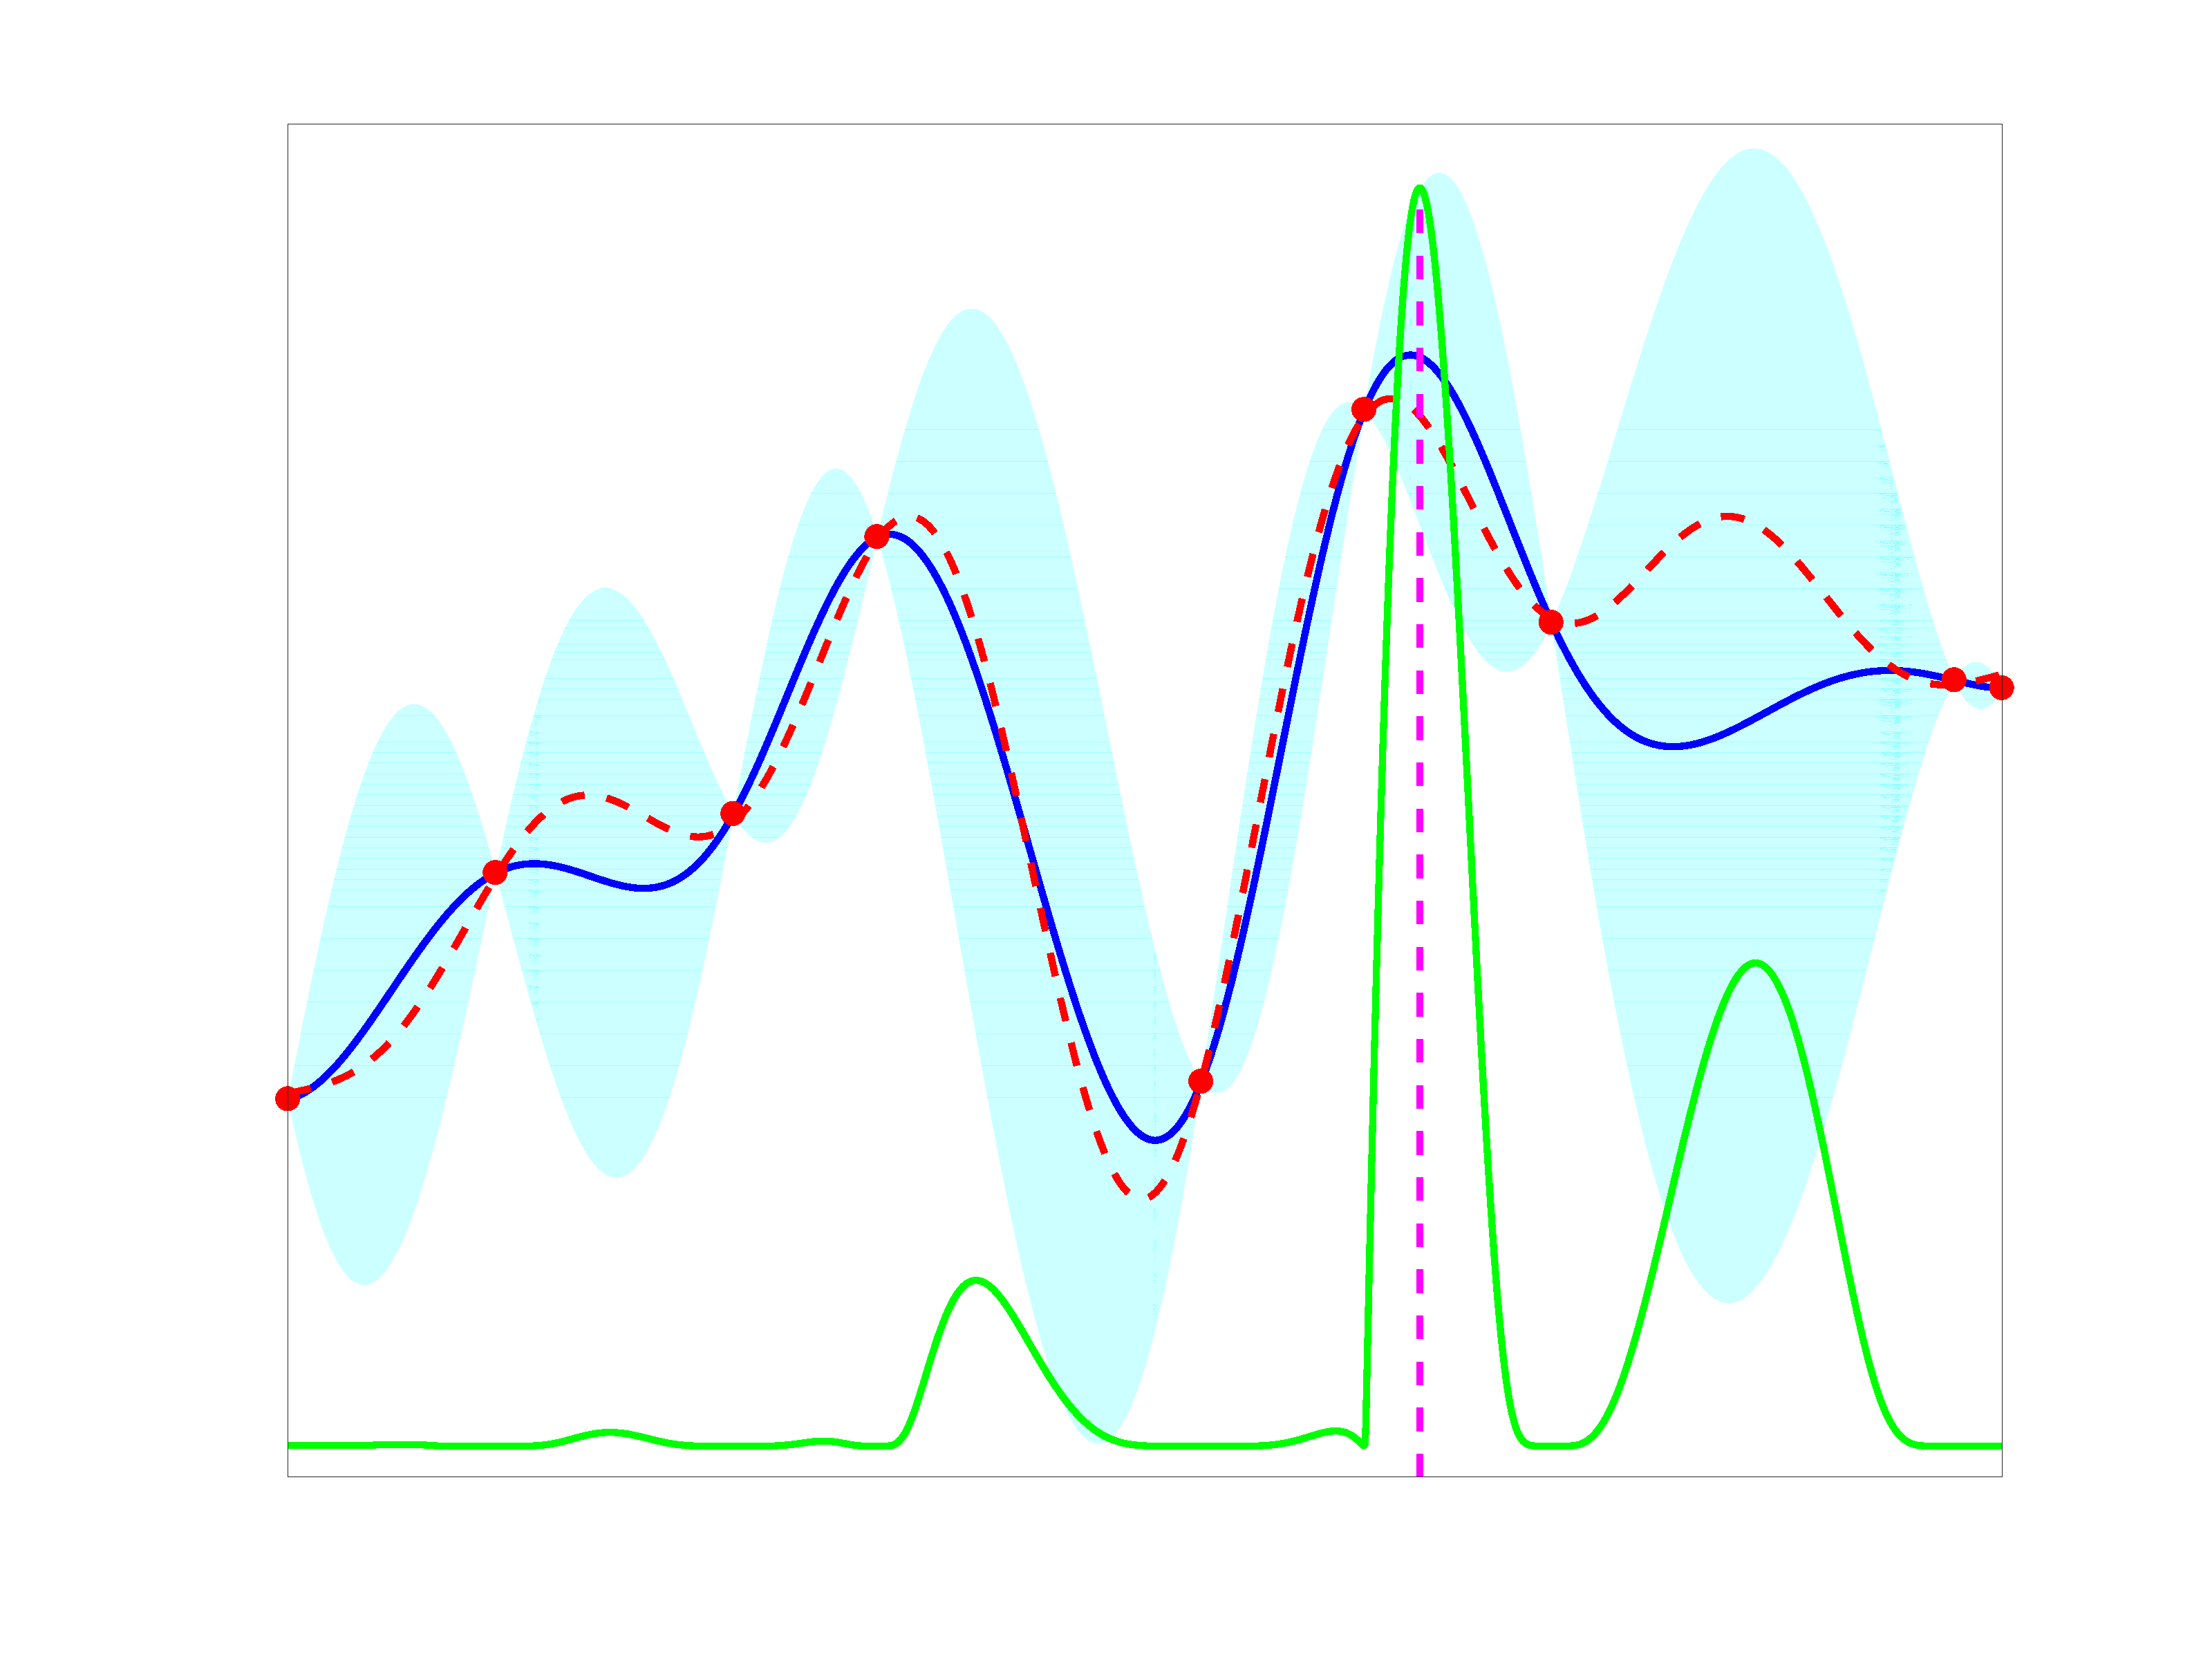
\includegraphics[width=0.6\textwidth]{10_with_acq_opt}
		\\
		11 Iterations & 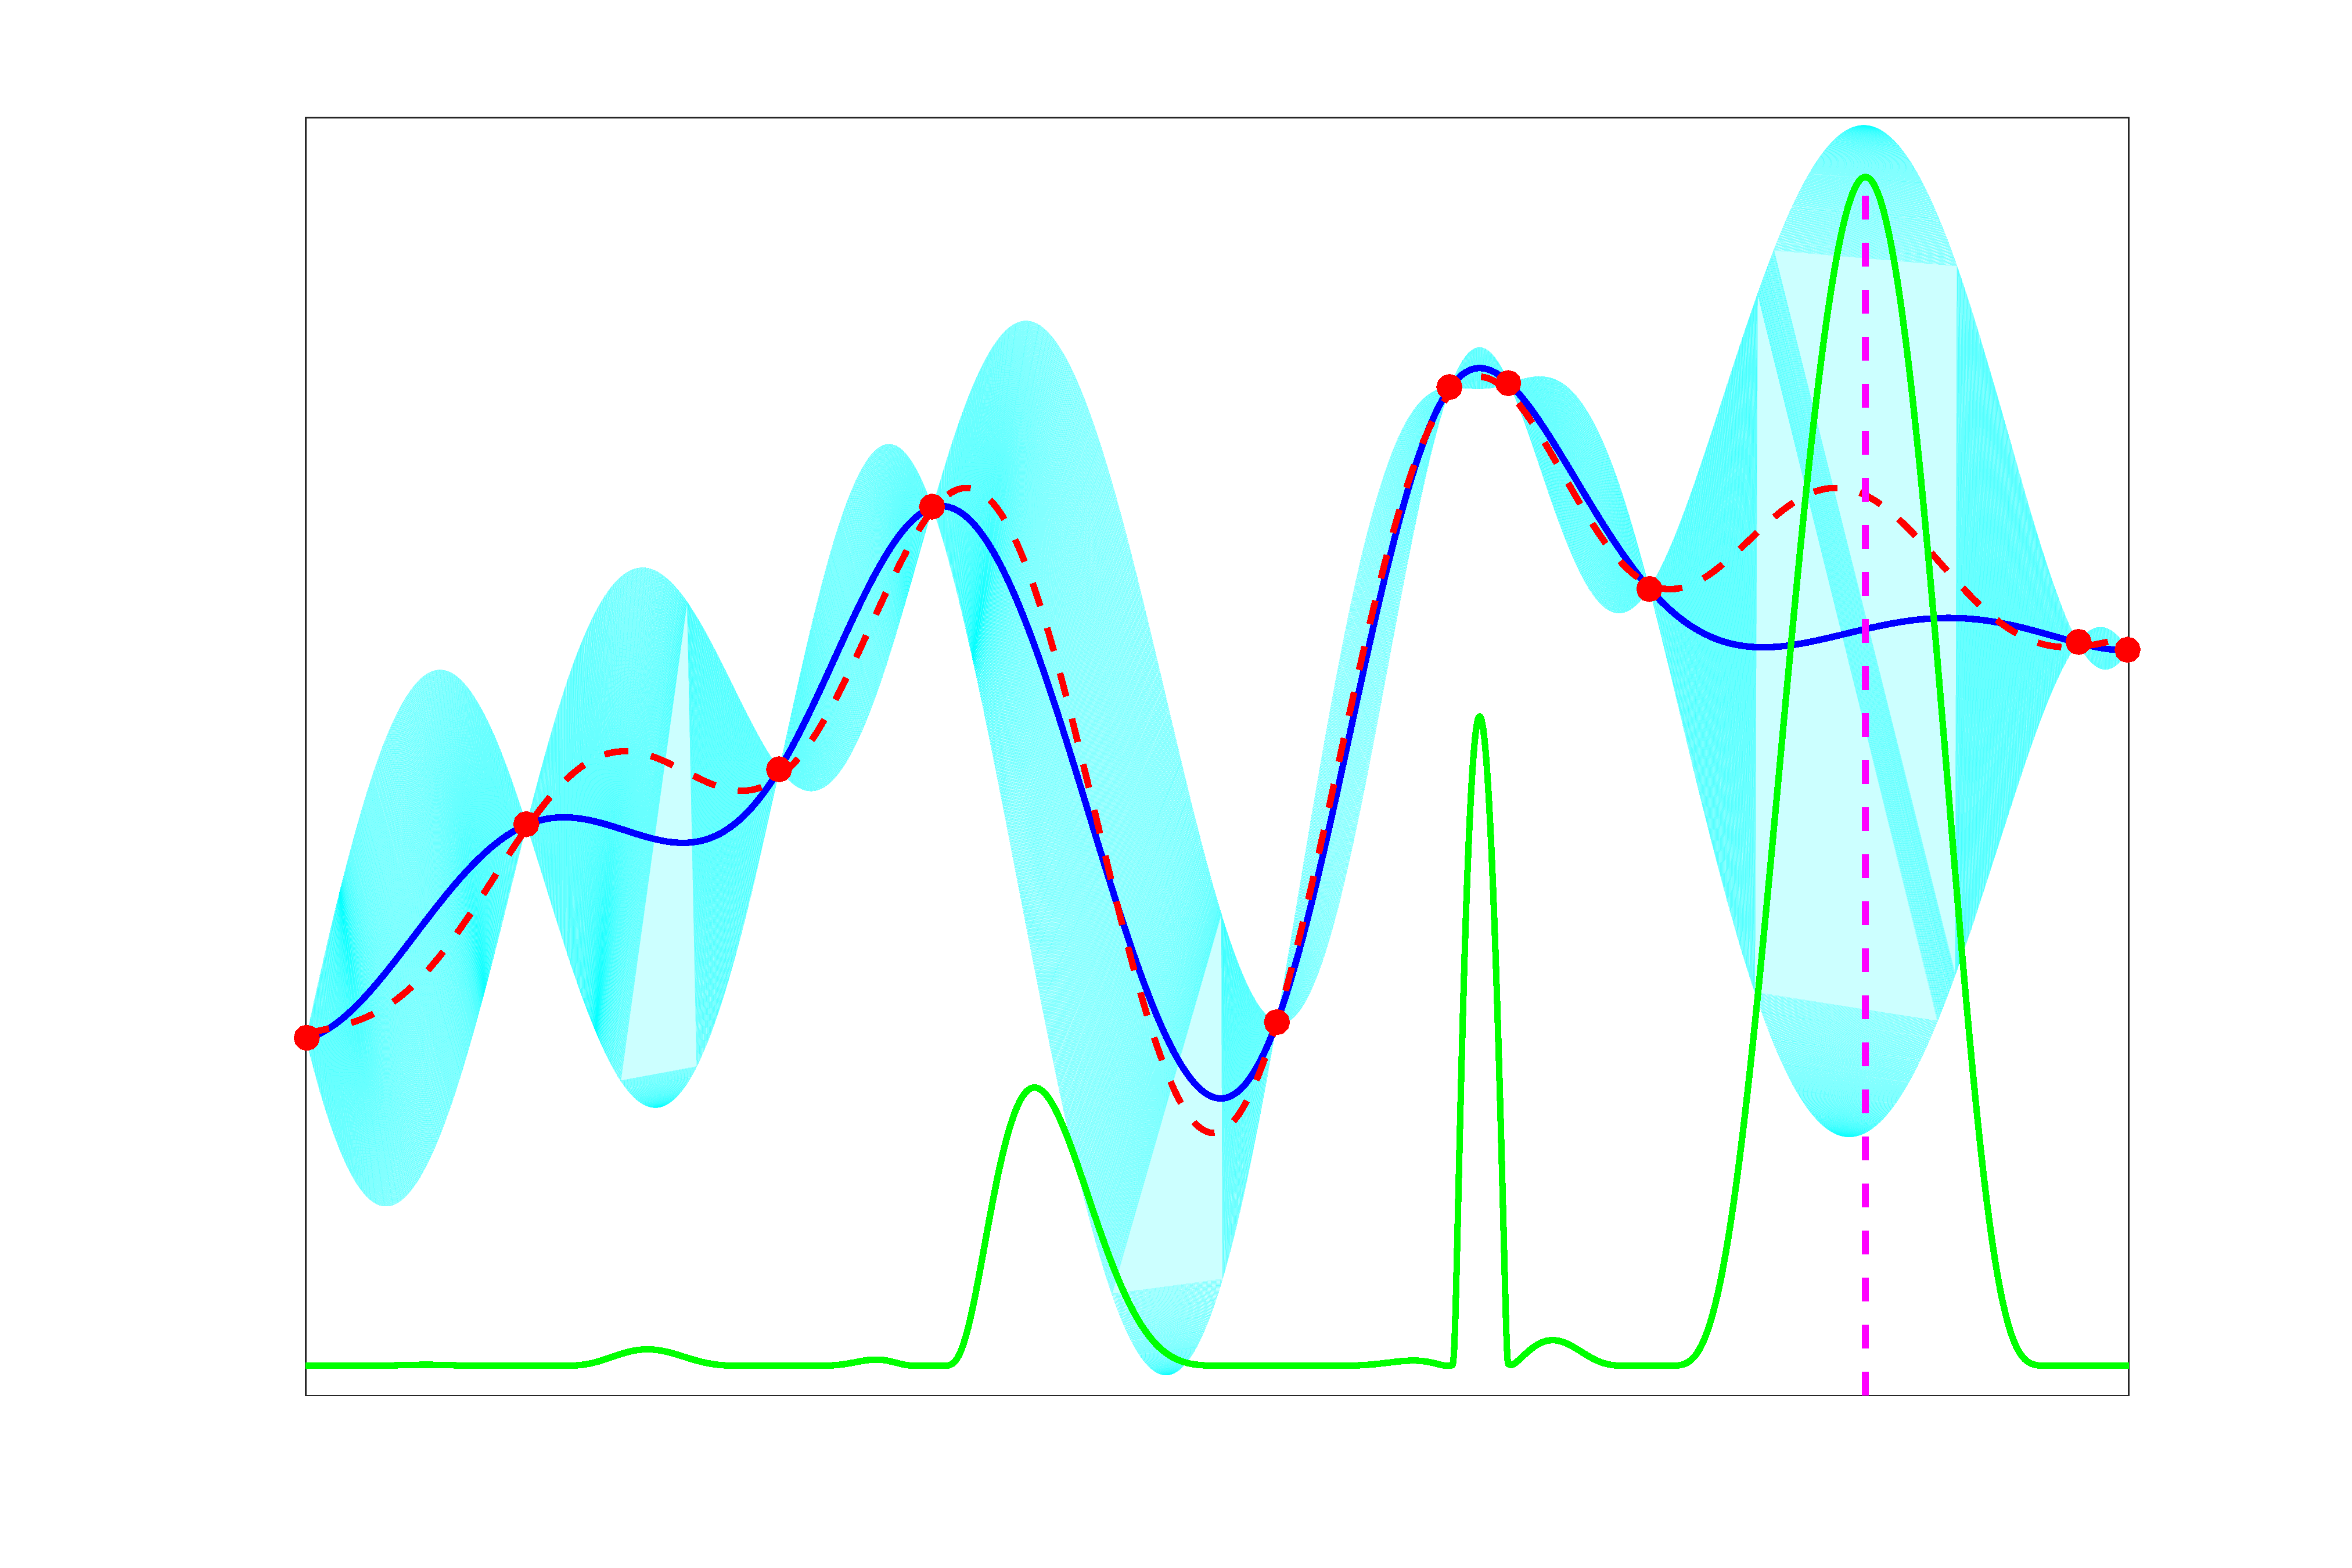
\includegraphics[width=0.6\textwidth]{11_with_acq_opt}
		\\
		20 iterations & 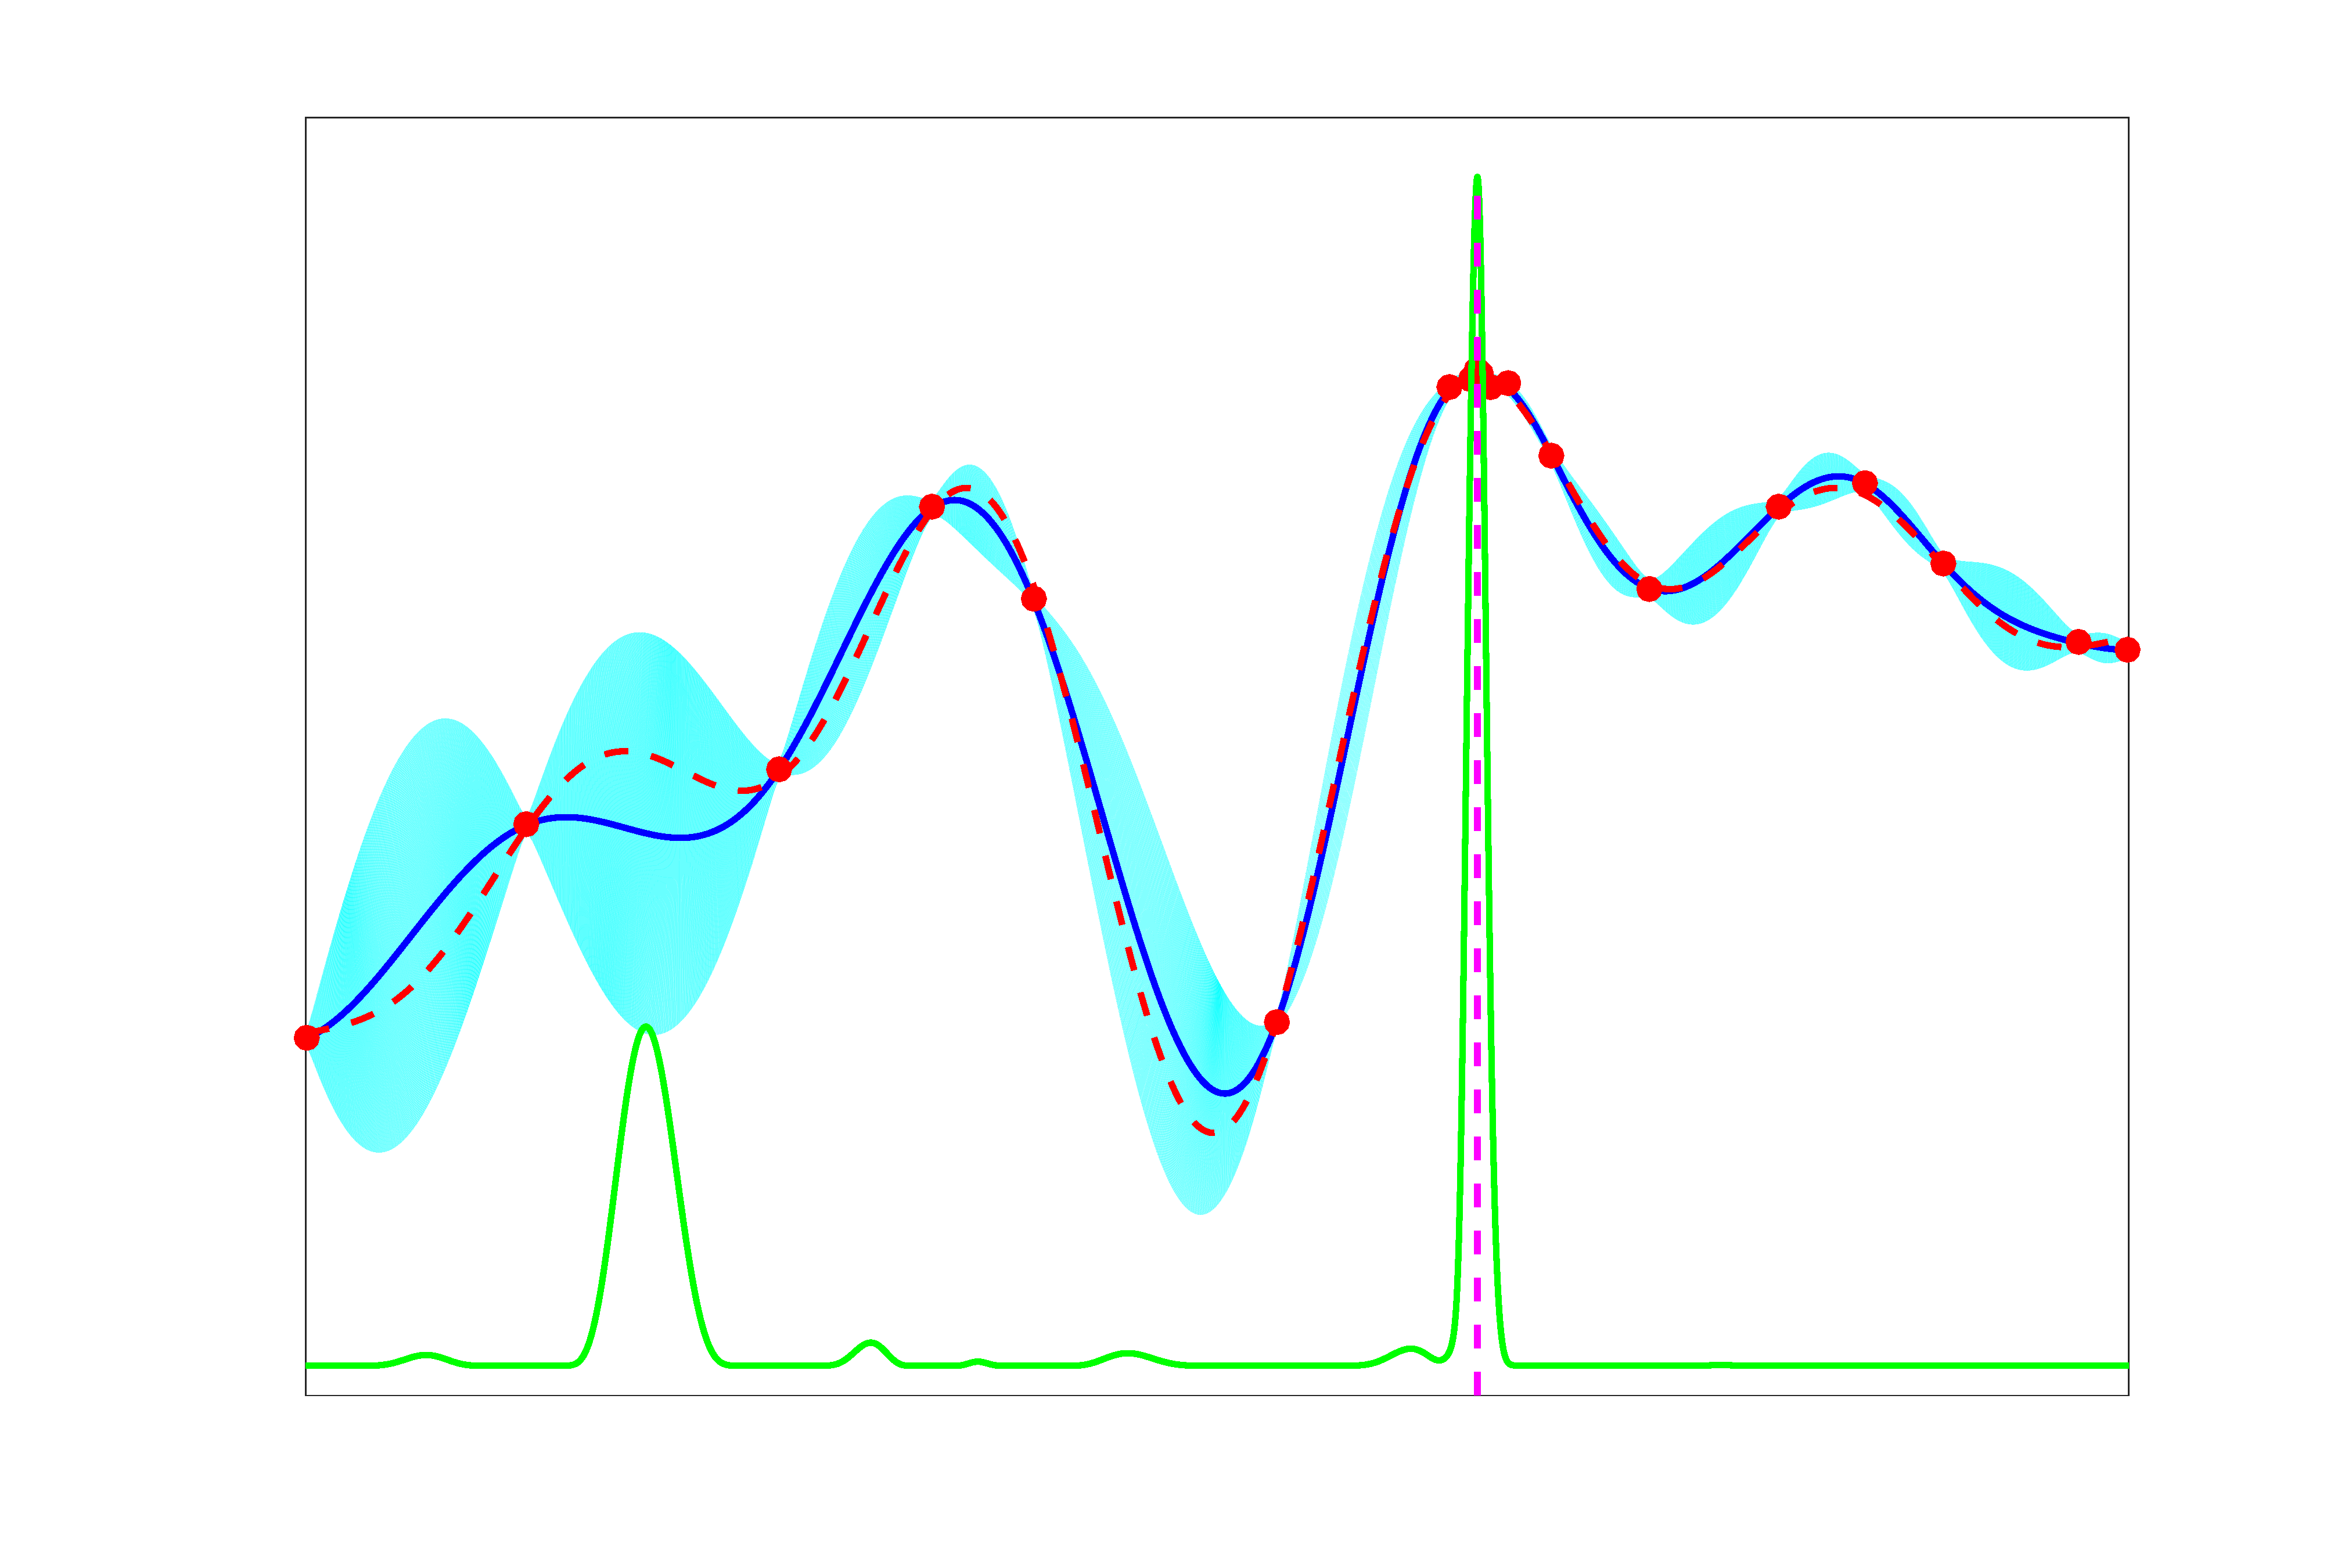
\includegraphics[width=0.6\textwidth]{20_with_acq_opt}
	\end{tabular}
	\caption{Illustration of using Bayesian optimization method to optimize the
		toy one dimensional problem given in~\eqref{eq:opt:toy}.  Red dots show
		the function evaluations,  the dotted red line shows the true function, 
		the solid blue line is the GP mean, the shaded region is the GP mean $\pm 2$
		standard deviations, the green line is the acquisition function, and
		the dotted purple line is the location of the maximum of the acquisition
		function. See main text for further description.\label{fig:opt:bayes-opt}}
\end{figure}

When prior information is known about the function, the
flexibility in choosing the covariance kernel can also be very helpful, for example allowing known
smoothness to be incorporated.  However, this can also be a curse as an inappropriate choice of
kernel can severely happen the performance.  In particular, it will typically be necessary to
do inference over, or at least optimize, the GP hyperparamters.  Another drawbacks to using GPs
is poor scaling in the number of iterations - training is a $O(N^3)$ operation due to the required
matrix inversion.  This typically restricts BO using GPs to using at most hundreds of iterations
unless appropriate approximations are made~\citep{snelson2006sparse,hensman2013gaussian}.
Another drawback can be poor scaling in the dimensionality of the inputs - most common kernels
rely on local modelling which can break down in high dimensions because points are typically
far away from one another \citep{bengio2006curse}.  

Figure~\ref{fig:opt:bayes-opt} shows BO being used to optimize the 
following simple one dimensional function
\begin{align}
\label{eq:opt:toy}
f(\theta) = \frac{\theta}{15}-\frac{\theta^2}{50}-\frac{\sin \theta}{\theta}, \quad -5\le \theta \le 5
\end{align}
with noisy observations $v\sim\mathcal{N}(f(\theta),0.01^2)$.  As we
explained before, BO employs only point-wise function
evaluations and so the optimization problem boils down to deciding 
\begin{enumerate}
	\item What input point should be evaluated at each iteration?
	\item Which point of those evaluated is most optimal?
\end{enumerate}
Both of these are done using a GP regressed to the existing evaluations,
which therefore forms the first step of each BO iteration.  As shown in
Figure~\ref{fig:opt:bayes-opt}, this gives an estimated value and uncertainty for the function
at every point in the form of the GP posterior mean $\mu_{\text{post}}(\theta)$ and 
marginal standard deviation $\sigma_{\text{post}}(\theta) = \sqrt{k_{\text{post}}(\theta,\theta)}$
where $\mu_{\text{post}}$ and $k_{\text{post}}$ are as per~\eqref{eq:opt:GP-posterior}.  We will
drop the $_{\text{post}}$ subscript in the rest of this chapter to avoid clutter.
The second decision is now straight forward - our
estimate for the most optimal point of those evaluated is simply the point with
the highest mean.  

To solve the first decision - where to evaluate next - we specify a so-called 
\emph{acquisition function}  $\zeta : \vartheta \rightarrow \real$
that encodes the relative utility of evaluating a new point.  The optimum of this
acquisition function is then the optimal point to evaluate at the next iteration.
At a high level, the utility
of a point is based on a trade off between \emph{exploration},
namely the desire to evaluate points where our uncertainty is high to reduce the
uncertainty in those regions, and \emph{exploitation}, namely the desire to evaluate points
where the expected function value is high so that we get a good characterization
of the function in promising regions.  One could alternative think about this as wanting to refine 
the estimates of promising local optima and sample in places that are likely to contain a
missing mode.
We will return to discuss specific acquisition
functions in depth in the next section and for now we simply note that the most
desirable points to evaluate will be those that provide both exploration and exploitation.
For example, consider the expected improvement acquisition function (see INSERT REF)
after 10 iterations shown in green in Figure~\ref{fig:opt:bayes-opt}.  This is reasonably
large in the two regions of highest uncertainty, but it is highest in the region near the 
true global optima where both
the expected value and uncertainty are high.  After 11 iterations on the other hand,
the uncertainty in this region has dropped dramatically and the point with the
highest uncertainty now has the largest value of acquisition function.  Note that
the scales for the acquisition function are different for the different iterations and
that the acquisition function typically decreases as more points are observed.

At first it might seem strange to replace our original optimization problem with
another in the form of optimizing the acquisition function to choose the point
to evaluate next.  This new optimization problem is itself a global
optimization of a typically highly multi-modal function and we need to carry it out
at each iteration of the BO algorithm.  Indeed if the target function $f$ is cheap to
evaluate, taking such an approach would be rather foolish.
The key difference though
is that surrogate optimization problem can be solved without the need to evaluate
the original target function.  Therefore, if $f$ is expensive to evaluate, this additional
computation can be justified if it keeps the number of required evaluations of $f$ to
a minimum.  There are also a number of other features that mean the problem of
optimizing the acquisition function is typically much easier than the original target --
it can be evaluated exactly, derivatives are often available, and provided an appropriate kernel
is used then it is guaranteed to be smooth.  It is also not typically necessary to ensure
that the acquisition function is optimized exactly, as evaluating a point that is
sub-optimal under the acquisition function simply means that a point expected to be less
helpful is evaluated at the next iteration.  This can be useful when the time for a BO
iteration is comparable to a function evaluation as the amount of computational effort
undertaken by the BO can be tuned to the problem at hand.  It is also worth noting that
the computational complexity for optimizing the acquisition function is theoretically less
(in terms of BO iterations) than the GP training ($O(N^2)$ instead of $O(N^3)$), though in
practice the two are typically comparable for the modest number of iterations BO is
generally run for.

Going back to Figure~\ref{fig:opt:bayes-opt}, we see that BO works by interleaving
regressing a GP to the evaluations, optimizing the acquisition function to find the next
point to evaluate, evaluating the target function at that point, and the updating the GP
regression again.  After 20 iterations for our simple problem, the GP regression around
the optimum has become very accurate, while it is less accurate elsewhere.  This
highlights the sample efficiency of BO as it shows how computational resources are
focussed on where they are required.

\subsection{Acquisition Functions}
\label{sec:opt:BO:acq}

As we previously explained, the GP posterior provides convenient analytic representations
for the expected value and uncertainty in the function in the form of the GP posterior mean 
$\mu (\theta)$ and marginal standard deviation $\sigma (\theta)$ respectively.  We now
introduce a number of common acquisition functions, many, but not all, of which will use
these representations directly.

The choice of acquisition function can be critical to the performance of Bayesian optimization
and its choice forms a basis for a significant proportion of the Bayesian optimization
literature~\cite{shahriari2016taking}.  In particular, some acquisition functions have
pathologies, for example a tendency to insufficiently explore, which can severely impede the
performance of BO.  This has lead to the development of some very powerful, but computationally
intensive and algorithmically complicated, acquisition strategies (e.g.~\cite{hernandez2014predictive}), 
such that there is often a speed / simplicity vs per iteration performance trade-off in their selection.

\begin{figure}[t]
	\centering
	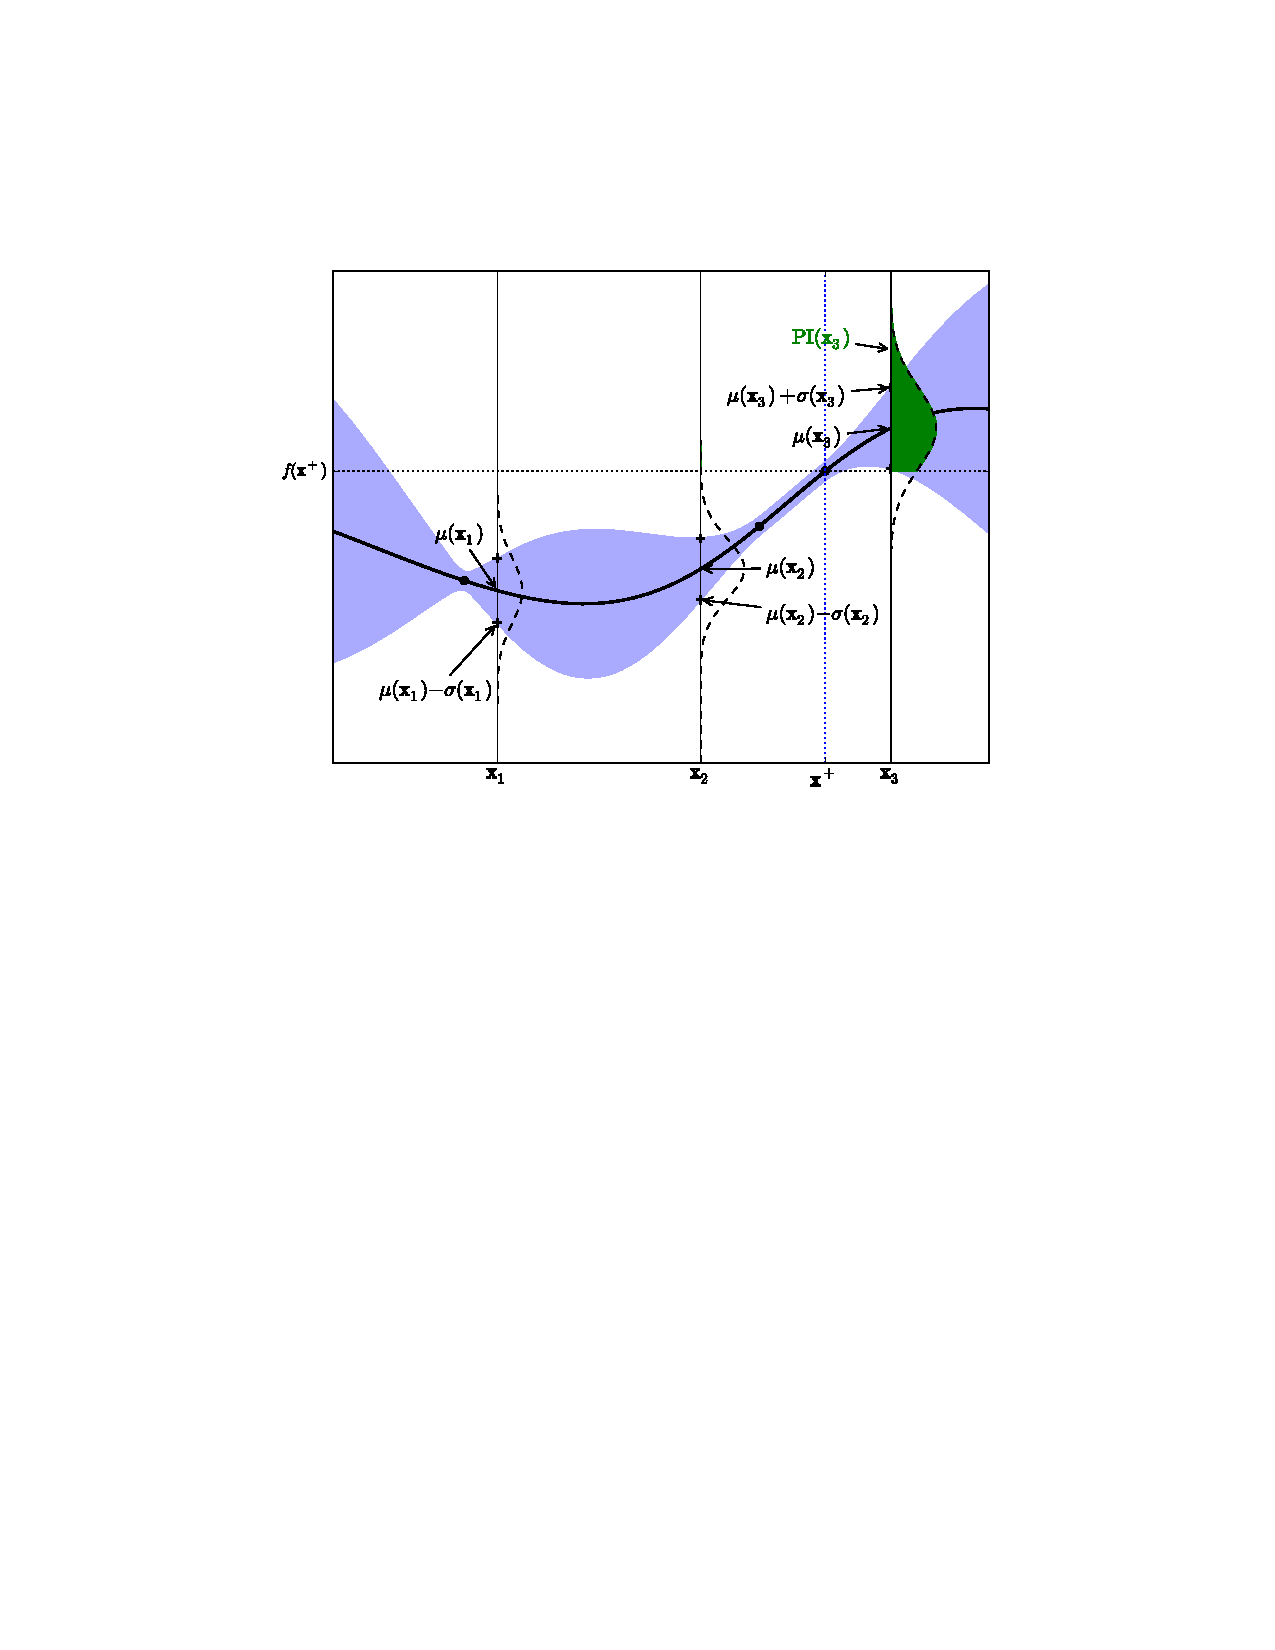
\includegraphics[width=0.95\textwidth]{prob_imp_brochu}
	\caption{Explanation figure for probability of improvement, taken from~\cite{brochu2010tutorial}.
		The best point so far (i.e. evaluated point with the highest GP mean) occurs at $\mathbf{x}^+$,
		with corresponding GP mean $\mu(\mathbf{x}^+)$ (for some reason $f(\mathbf{x}^+)$ is shown
		instead).  The probability of improvement at any point corresponds to the marginal probability that the 
		the true function value at that point is larger than $\mu(\mathbf{x}^+)$.  An example of which is 
		shown at the point $\mathbf{x}_3$, corresponding to the green shaded region, which is clearly
		substantially larger than at two other hypothetical points $\mathbf{x}_1$ and $\mathbf{x}_2$.
		Note also that the expected improvement of $\mathbf{x}_3$ corresponds to the expectation 
		of $\mathbf{x}_3-\mathbf{x}^+$ under the distribution of the green shaded region, while the 
		point $\mu(\mathbf{x}_3)+\sigma(\mathbf{x}_3)$ corresponds to the UCB acquisition function
		with $\kappa=1$.
		REPLACE WITH OWN FIGURE\label{fig:opt:prob-imp}}
\end{figure}

\subsubsection{Probability of Improvement}
\label{sec:opt:BO:acq:prob}

One of the conceptually simplest acquisition functions is the probability of improvement (PI, \cite{kushner1964new}), namely
the probability that the function value at a point is higher than the current estimated optimum.  A
characterization of this is shown in Figure~\ref{fig:opt:prob-imp}.  As shown by, for example,
\cite{brochu2010tutorial}, the probability of improvement has a simple analytic form because the
marginal distributions for function evaluations are Gaussian.  Specifically, let
\begin{align}
\label{eq:opt:muplus}
\mu^+ = \max_{j\in \{1,\dots,m\}} \mu\left(\theta_j\right)
\end{align}
denote the point with the highest expected value and define
\begin{align}
\label{eq:opt:gamDef}
\gamma\left(\theta\right) = \frac{\mu \left(\theta\right)-\mu^+-\xi}{\sigma\left(\theta\right)},
\end{align}
where $\xi \ge 0$ is a user set parameter ($\xi=0$ in Figure~\ref{fig:opt:prob-imp}).
The probability of improvement is then defined as the probability of improving the 
objective function by at least an amount $\xi$
\begin{align}
\label{eq:opt:PI}
\mathrm{PI}\left(\theta\right) = p \left(f\left(\theta\right)\ge \mu^+ +\xi\right) = \Phi \left(\gamma\left(\theta\right)\right)
\end{align}
where $\Phi \left(\cdot\right)$ represents the unit normal cumulative distribution function.  
Note that $\xi=0$ corresponds to pure exploitation and $\xi \rightarrow \infty$ 
corresponds to pure exploration.  Typically for PI, one will employ a cooling schedule 
for $\xi$ to incorporate the intuitive idea that one should first explore and then 
exploit.  However, as shown by for example \cite{jones2001taxonomy}, 
the performance of the PI acquisition function is sensitive to the choice of 
$\xi$ and therefore the cooling strategy requires careful tuning.  Doing this in effectively in
a general purpose way is very challenging, meaning that PI
is rarely used in practice.

\subsubsection{Expected Improvement}
\label{sec:opt:BO:acq:expt}

A method less sensitive to tuning is the expected improvement~\citep{movckus1975bayesian}.  
It is conceptually similar to PI, but incorporates the idea that large improvements are more beneficial
to small improvements. It therefore better represents the importance of exploration and
is less prone to over-exploitation.
It can also be calculated analytically for a GP (see e.g. \cite{brochu2010tutorial}) leading to
the following definition
\begin{align}
\label{eq:opt:EI}
\begin{split}
\mathrm{EI} \left(\theta\right) = & \int_{\mu^+ +\xi}^{\infty} p\left(f\left(\theta\right)|\mu\left(\theta\right),\sigma\left(\theta\right)\right) \left(f\left(\theta\right)-\mu^+-\xi\right) df\left(\theta\right) \\
= & \begin{cases}
\left(\mu\left(\theta\right)-\mu^+-\xi\right)\Phi \left(\gamma\left(\theta\right)\right)+\sigma\left(\theta\right)\phi\left(\gamma\left(\theta\right)\right), & \sigma \left(\theta\right) > 0 \\
0, & \sigma \left(\theta\right) = 0
\end{cases}
\end{split}
\end{align}
were $\phi \left(\cdot\right)$ represents the probability density function of the unit normal distribution.  
The parameter $\xi$ plays a similar role as for the PI, but in this case $\xi=0$ no longer corresponds 
to pure exploitation.  \cite{lizotte2008practical} suggests that cooling schedules on $\xi$ are 
not helpful for EI and that $\xi = 0.01 \mathbb{E} \left[\sigma \left(\theta\right)\right]$ where 
$\mathbb{E} \left[\sigma \left(\theta\right)\right]$ is signal standard deviation works well in almost all cases.
Simply setting $\xi=0$ is also a common choice, but it can be prone to doing insufficient exploration.
Convergence rates for EI have been demonstrated by~\cite{bull2011convergence}.

\subsubsection{Upper Confidence Bounding}
\label{sec:opt:BO:acq:ucb}

Another possible acquisition strategy is to maximize the upper confidence bound (UCB) for
the function value~\citep{lai1985asymptotically,srinivas2009gaussian}, namely
\begin{align}
\label{eq:UCB}
\mathrm{UCB}\left(\theta\right) = \mu \left(\theta\right) + \kappa \sigma \left(\theta\right)
\end{align}
where $\kappa \ge 0$ is again a parameter that will control the exploration / exploitation trade off.
This bound represents point at which the probability the function is less than this value is $\Phi (\kappa)$.
A particularly nice feature of the UCB acquisition function is that given certain constraints on 
$\mX$ and $k$, $\kappa$ can be chosen in a manner such that acquisition has bounded 
cumulative regret with high probability, this is known as GP-UCB \citep{srinivas2009gaussian}. 
However, the need to (often adaptively) set $\kappa$ can be a noticeable drawback.

\subsubsection{Information-Based Policies}
\label{sec:opt:BO:acq:inf}

At the end of the day, the aim of BO is to find the location of the optimum.  The true utility of
evaluating a new point is, therefore, in the information it provides about the location of the
true maximum $\theta^*$ and the assistance it provides in guiding future evaluations.  Though 
the latter of these is difficult to actively incorporate, the former is something that can be
target in a principled manner by considering the distribution on the location of the maximum
$p(\theta^* | \Theta, V)$ where $\Theta$ and $V$ are the previously evaluated input and output
points as per Section~\ref{sec:opt:GPs}.

The simplest way this can be done is using Thompson sampling\cite{thompson1933likelihood}, 
where instead of optimizing an acquisition function directly, one looks to sample the next
point to evaluate from $p(\theta^* | \Theta, V)$~\citep{shahriari2014entropy,kandasamy2017asynchronous}.  
In the GP setting, this is equivalent to sampling a particular function realisation $f$ and then taking 
$\theta_{\text{next}}$
as the optimum of this particular realisation.  This can prove surprisingly expensive, as sampling
a joint realisation of a GP at $M$ points is an $O(M^3)$ operation.  

A more complicated, but theoretically more powerful approach, is to try and directly optimize
for the point that will, in expectation, most reduce the uncertainty about the location of the maximum.
These so called entropy search (ES) methods 
\citep{villemonteix2009informational,hennig2012entropy,hernandez2014predictive} use as an
acquisition function the expected gain in Shannon information about the location of the optimum,
or equivalently the reduction in entropy of the location of the maximum. Namely they take
\begin{align}
\label{eq:opt:ent-search}
\zeta (\theta) = H\left[p(\theta^* | \Theta, V, \theta)\right]-
\E_{p(v| \Theta,V, \theta)} \left[H\left[p(\theta^* | \Theta, V, \theta, v)\right]\right]
\end{align}
where $H[p(x)]=-\int p(x)\log p(x)dx$ is the differential entropy of its argument
and $p(v| \Theta,V, \theta)$ is the predictive distribution of the GP such that
$v\sim\mathcal{N}\left(\mu(\theta),\sigma(\theta)^2+\sigma_n^2\right)$ as
explained in Section~\ref{sec:opt:GPs:function}.
Entropy search methods are closely linked to the idea of Bayesian experimental design, in which an equivalent
target has been used for some time~\cite{chaloner1995bayesian}.  We return to Bayesian experimental
design in detail in Chapter INSERT.

Unfortunately,~\eqref{eq:opt:ent-search} is not analytically tractable and so entropy
search methods must rely on methods for approximately solving~\eqref{eq:opt:ent-search}.  
This can be particularly difficult as~\eqref{eq:opt:ent-search} represents a nested estimation
problem that cannot be solved simply by, for example, Monte Carlo~\citep{rainforth2016pitfalls}.
An important advancement in this regard was the development of an estimation scheme
by~\cite{hernandez2014predictive} that uses a combination of analytic approximations
and Monte Carlo sampling.  Despite these approximations, the resulting predictive ES algorithm
provides excellent empirical performance in terms of the number of function 
evaluations and remains arguably the state-of-the-art acquisition function for BO.

\subsubsection{Other Acquisition Functions}
\label{sec:opt:BO:acq:other}

Many more acquisition strategies have been developed than we have space 
to cover here.  However, some of other strategies of particular note include
\begin{itemize}
	\item \cite{contal2014gaussian} construct an acquisition function from a combination
	of the GP mean and an approximation of the mutual information between the
	function and the noisy evaluations at the chosen input points.  This leads to impressive
	theoretical and empirical results.
	\item \cite{osborne2009gaussian,gonzalez2016glasses} develop
	non-myopic methods that incorporate the effect of future hypothetical evaluations on
	the relative optimality of evaluating a point at the current iteration.  Such lookahead methods
	can improve performance, but at the expensive of substantially increased computational cost.
	\item \cite{wang2016optimization} introduce a strategy explicitly estimating then using
	the value of function maximum $f(\theta^*)$ and establish links connections between their
	approach, UCB, and PI.
	\item \cite{swersky2013multi,shah2016pareto,hernandez2016predictive,feliot2017bayesian}
	introduce various acquisition functions for dealing with multi-objective problems where we
	wish to optimize many functions simultaneously.  For example, they may try to approximate
	the so-called Pareto front, constituting of the set of non-dominated solutions.
\end{itemize}

\subsection{GP Hyperparameters}
\label{sec:opt:BO:hyp}

Generally the performance of BO will be strongly dependent on the choice of GP
 hyperparameters $\alpha$.  Rather than optimizing for $\alpha$ it is natural, 
 when tractable, to take a fully Bayesian view and marginalize
 over $\alpha$ \cite{osborne2009gaussian, snoek2012practical}, leading to
 mixture of GPs posterior.  This was shown
 by~\cite{snoek2012practical} to substantially improve the performance of BO.
 An easy way to do this for simple acquisition functions is to consider an
 integrated acquisition function corresponding to the expectation of the acquisition
 function over the GP hyperparamters~\citep{snoek2012practical}
\begin{align}
\label{eq:opt:intAcq}
\bar{\zeta}\left(\theta \right) &= \E_{p\left(\alpha | \Theta, V\right)}
\left[  \zeta\left(\theta  ; \alpha\right)  \right] \\
&= \frac{1}{p\left(V | \Theta \right)} \E_{p\left(\alpha \right)}
\left[  \zeta\left(\theta  ; \alpha\right)  p\left(V | \Theta, \alpha\right)\right]
\end{align}
where $p(\alpha)$ is a prior over the hyperparmaeters, $p\left(V | \Theta \right)$ is
a constant that can be ignored as it does not effect the position of the optimum, and
$p\left(V | \Theta, \alpha\right)$ is GP marginal likelihood as given in~\eqref{eq:opt:GP-ML}.
The expectation can be approximated using Monte Carlo inference, with slice sampling
\citep{neal2003slice,murray2010slice} and Hamiltonian Monte Carlo \citep{duane1987hybrid,hensman2015mcmc}
being common choices.

\subsection{Extensions and Practicalities}
\label{sec:opt:BO:exten}

\subsubsection{Constraints}
\label{sec:opt:BO:exten:constraints}

Bayesian optimization approaches have mostly assumed that the target function
is constrained by a bounding box, i.e. that each input is independently constrained.
In practice, this is assumption is rarely fulfilled exactly, though for technically unbounded 
problems then it is not uncommon
for the user to be able to specify a box conveying the region where it is reasonable to
assume to the true optimum falls within the box.  To go beyond this assumption, it is
necessary to design strategies that can deal with constraints.
